%!TEX root = ../main.tex

This section covers the steps needed to produce the wanted results. The input needed is a fiducial marker M to provide the object position in the real world; and a 3D mesh O which will be rendered in Augmented Reality. The output is a set of light sources L\textsubscript{i}, each one having a position, orientation, intensity, color, type and size. In order to complete the luminance (luma) analysis a 360 panoramic image is required, but it will be generated as a previous step, it is not necessary to have one beforehand. The entirety of the process is layed out in the flowchart in Figure 1, and each step is described in more detail afterwards.

\begin{figure}[H]
  \centering
  \setlength{\unitlength}{\textwidth} 
    \begin{picture}(1,0.5)
       \put(-0.1,0){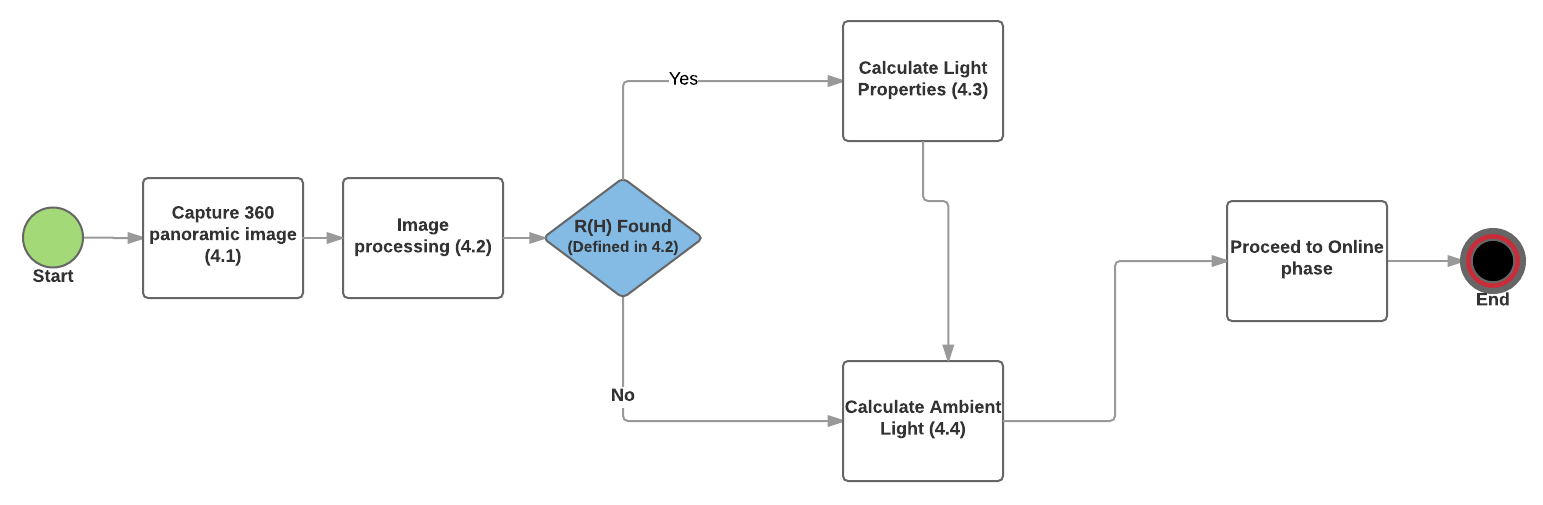
\includegraphics[width=1.3\unitlength]{Figures/Flowchart.png}}
       
    \end{picture}
    \caption{The method in a nutshell}
\end{figure}

\subsection{Panoramic image capture}
In this work panoramic images are used as a tool, therefore it's not within the scope of the method to define a new way of capturing 360 images. The implementation will be based on the one by Chuang et al. \cite{ThreeSixty}
M will provide the origin of the virtual world for placing and orienting O within it. In order for the lights to be mapped to the same position as M the user will be asked to place the marker in the desired position and start capturing the environment while the marker is centered in frame. This will also simplify calculations of light orientations later on.

\subsection{Image processing}
Once the panoramic image exist the first step in order to be able to analyze the luminance is to get rid of the chromatic information. This is achieved with the following equation:
\[
    L(R_{ij},G_{ij},B_{ij}) = 0,2126 \times R_{ij} + 0,7152 \times G_{ij} + 0,0722 \times B_{ij}; \quad \forall \  P_{ij}
\]
Where L is the luminance obtained at D65 white point, which corresponds roughly to the average midday light in Western Europe / Northern Europe; and P is the pixel in the i,j position of the image \newline
The contrast ratio has to be adjusted, so that the regions with high luminance are more clearly differentiable. 
\[
    g(i,j) = \alpha \times f(i,j) + \beta
\]
Where g(i,j) is the adjusted image, f(i,j) is the original grayscale image and $\alpha$ and $\beta$ are the brightness and contrast constants, determined by parameter tuning.
In order to prevent outlier pixels and noise from causing false positives, let g(i,j) be normalized like so:
\[
    L(P_{ij}) = \frac{ 2 \times P_{ij} }{min_{ij} + max_{ij}}
\]
Where min\textsubscript{ij} and max\textsubscript{ij} are the overall minimum and maximum luminance values in the image. 
\newline
The result of these steps is a black and white image with the rough shape of the light source. If the image ends up completely black it means there are no important visible light sources and ambient illumination alone would give a good enough result on the rendered model. A region of high luminance is defined as follows:
\[
    R(H) = \{p_{00}, p_{01}, ... , p_{mn}\}
\]
 Where p\textsubscript{ij} is the pixel in the i,j position of the image. Such that 
\[
    L(p_{ij}) > 0.9 \times max(L(p_{ij})) 
\]
However if there are regions of high luminance they would be discovered with a fair amount of noise and artifacts, caused by clear objects, reflections of light sources on highly reflective surfaces, or even light sources that are so far away in the distance that don't really contribute an important amount of light to the area of interest. Therefore it's necessary to also add a relative size constraint to the definition. What constitutes an acceptable region size to deem the light source is not an easy question to answer. The best approach to face this problem is to define it as a percentage of the width and height of the overall image and tune the parameter in search for the best solution. The size constraint would therefore be:

\[
    width(R(H)) \times height(R(H)) \geq k \times W \times H
\]
Where k is the parameter to be tuned; W and H are the total image width and height.\newline

These constraints also help keep the amount of lights to be processed within an acceptable range for a real-time application, even if the real environment has many light sources a simplification of them is necessary when modelling them to keep the application feasible. Once the relevant light sources have been identified their properties need to be calculated.

\subsection{Calculate light properties}
The properties needed to calculate for each light are position, orientation, intensity, size and color. In the real world it is not trivial to calculate the position and size at the same time, because at least one of them would have to be known. Fortunately in the virtual world this is not necessary, as long as it is consistent, for the area size of the light the pixel measures can be used. With this in mind all the other properties can be calculated.

\begin{enumerate}
\item Width and height: The pixel measures will be used for this, they can me determined from the size constraint in the previous step.
\item Position: It is posible to calculate the distance from and object to a camera lens knowing a few parameters from the lens, namely the focal lenght and the sensor size. In Android these values are easily obtainable through the ExifInterface class. In iOS the values are publicly known per device family, so it's possible to create a lookup table with the values and have the application ask what device it's running on to match the necessary set of values. The calculation is then done as follows:
\[
    d(L_i) = \frac{ f \times h_i}{sensorHeight}
\]
\item  Orientation: Since the user was enforced to capture the environment starting from the north and the environment is the entire 360 degrees it is easy to map the pixel width to the angle of incidence of the light source. We can for example define the following ratio to calculate the angle:
\[
    \phi = \frac{pos(L_i)_x \times 180}{imageWidth \times 0.5}
\]
\item Color: Storing both versions of the panorama, one in full color and another one after processing will allow us to have both the color and the luminance information. Once a light source is detected, the equivalente area in the color image can be averaged to determine the color of the light source.
\item Type: There are two main shapes of lamps in the real world, quadrilateral and elliptical. It is indeed possible to find lights with more complex shapes, however, as long as the area of emission is the same, simplifying it to a quadrilateral or elliptical shape yields the same result for the purposes of the method.
\newline 
Determining if the light is a spotlight or an area light will be done through the shape. Elliptical lights will be tagged spotlights and quadrilateral lights area light. Shape detection will be carried out using OpenCV contour detection and counting the vertices of the contour. Even if in the real world the light is a perfect square and the camera is facing it with no parallax it is expected that,  due to artifacts and noise, the function may not find exactly 4 vertices. This is not a big problem, because the number of vertices needed to create smooth circle range in the dozens. So adjusting a threshold value is a simple and acceptable solution.
\end{enumerate}

\subsection{Calculate ambient light}
Since the data from the device's sensors are available something more involved than having a default value of ambient illumination for the entire scene. Ambient illumination when no visible light sources are present is more often than not due to sunlight, be it in an outdoors scene or coming in from a window somewhere. There are ways \cite{solar} to calculate the sun position in spherical coordinates using the latitude, longitude, time of the day and day of the year of the observer. This information can be easily retrieved using the devices GPS, clock and calendar. The direction in which the sunlight is affecting the scene can be used in a per-vertex illumination shader to adjust the amount of ambient light in a specific vertex of the virtual object. This contribution can be done using lambertian diffuse contribution:
\[
    I_a = K_a \times (N \cdot L)
\]
Where $K_a$ is the maximum ambient contribution, N is the vertex normal and L is the light direction vector, normalized.